\begin{center}
\textit{Bizon, Gorbahn, Haisch, Maltoni, Pagani, Shivaji, Zanderighi, Zhao}
\end{center}

In this section we discuss the possibility of indirectly extract information on the trilinear self interaction of the Higgs boson via precise measurements of single-Higgs production~\cite{McCullough:2013rea,Gorbahn:2016uoy,Degrassi:2016wml,Bizon:2016wgr,DiVita:2017eyz,Barklow:2017awn,Maltoni:2017ims,DiVita:2017vrr,Maltoni:2018ttu} at the HL-LHC and HE-LHC. This strategy is complementary to the direct measurement via double-Higgs production, which already at leading order,~i.e.~at one loop in the case of $gg \to HH$, depends on the trilinear Higgs self interaction. In the case of single-Higgs production, on the contrary, the Higgs self interactions enter only via one-loop corrections, i.e., at the two-loop level for the gluon-fusion ($ggF$) production mode. The effects of modified Higgs self interactions are therefore generically much smaller, but for single-Higgs production processes the precision of the experimental measurements is and will be much better than for double-Higgs production. This, and the fact that for single-Higgs production many different final states and both inclusive as well as  differential measurements are possible will lead to competitive indirect determinations of the trilinear Higgs self coupling. In \cite{Degrassi:2017ucl,Kribs:2017znd} also electroweak (EW) precision observables have been considered to this purpose.

In the following subsection, we will briefly recall the calculation framework introduced in~\cite{Gorbahn:2016uoy,Degrassi:2016wml}. We also provide  numerical results for the effects due to a modified  trilinear Higgs coupling in the most important inclusive and differential single-Higgs production cross sections as well as the Higgs branching ratios. Based on these results, we will analyse the sensitivity of the HL-LHC and HE-LHC in constraining the trilinear Higgs self interactions. 

\subsubsubsection{Theoretical framework}
\label{tril-single:theo}

The effects of anomalous Higgs interactions can be extracted from experimental data via the signal strength parameters $\muif$, which
are defined for any specific combination of production and decay channel $i \to H \to f$ as follows 
\be \label{signalstre}
\muif \equiv \mu_i \times \mu^f = \frac{\sigma(i)}{\sigma^{\rm SM} (i)} \times \frac{\br(f)}{\br^{\rm SM}(f)} \, .
\ee 
Here the quantities $\mu_i$ and $\mu^f$ are   the production cross sections $\sigma(i)$ ($i=$ $\ggF$, {\rm VBF}, $WH$, $ZH$, $t \bar tH$, $tHj$) and the branching ratios $\br(f)$ $(f= \gamma\gamma, ZZ, WW, b\bar{b}, \tau\tau, \mu\mu)$ normalised to their SM values, respectively. Assuming on-shell production, the product $\mu_i \times \mu^f$  therefore corresponds to the rate for the $i \to H \to f$ process  normalised to the corresponding SM prediction.

The quantities $\mu_i$ and $\mu^f$ that enter the definition of  $\muif$ in~(\ref{signalstre})  can be expressed as
\begin{equation} \label{eq:muf}
\mu_i = 1 + \dsigmah(i) \,,  \qquad 
\mu^f = 1 + \dBR(f) \,,
\end{equation}
where $\dsigmah(i)$ and $\dBR(f)$ are the deviations induced by an anomalous trilinear Higgs self interaction to the production cross sections and branching ratios, respectively.
This definition can be straightforwardly extended to the differential level and one has $\muif=\mu_i=\mu^f=1$ in the~SM.

In single-Higgs production, the trilinear Higgs self interactions start to enter only at the one-loop level in the case of vector boson fusion (VBF), $WH$, $ZH$, $t \bar tH$, $tHj$ production, while in the case of $\ggF$ production and the decays $H\to gg, \gamma \gamma$ one has to calculate two-loop EW corrections. The appearance of the quadrilinear Higgs self coupling in single-Higgs processes is further delayed by one loop order.

For the strategy discussed here, the anomalous trilinear Higgs self interactions can be equivalently parameterised either via an anomalous trilinear coupling  
\begin{equation}
\tril \equiv \ktre \trilsm
\end{equation}
where $\lambda_3^{\rm SM} = m_H^2/(2 v^2)$ with $v = (\sqrt{2} G_F)^{-1/2} \simeq 246 \, {\rm GeV}$ the EW vacuum expectation value, or via the corresponding dimension-six operator 
\begin{equation} \label{O6}
{\cal O}_6 = - \frac{\lambda_3^{\rm SM} c_6}{v^2} \, |\Phi|^6  \,,
\end{equation}
with $\Phi$~denoting the usual SM Higgs doublet. In the normalisation adopted in (\ref{O6}), the simple relation 
\begin{equation}
\ktre = 1 + c_6 \,,
\end{equation}
is obtained and allows to translate constraints on the coupling modifier $\ktre$ into bounds on the Wilson coefficient $c_6$ and vice versa. 

\begin{figure}
	\centering
	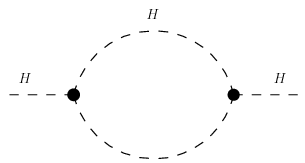
\includegraphics[width=0.45\linewidth]{\main/section3/plots/figDGMP_HiggsSelf1.png}\\
	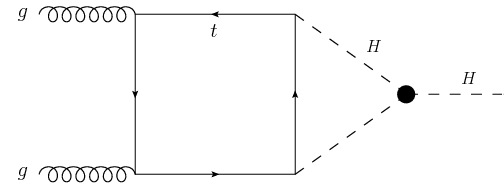
\includegraphics[width=0.45\linewidth]{\main/section3/plots/figDGMP_Hgg2.png}
	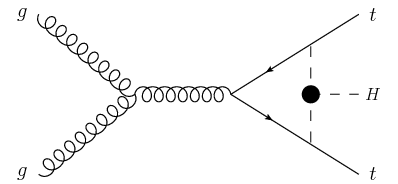
\includegraphics[width=0.45\linewidth]{\main/section3/plots/figDGMP_Htt2.png}
	\caption{Examples of NLO contribution of the Higgs self-coupling to single Higgs observables. Top: Contribution to the Higgs self-coupling, which generates a global correction to all amplitudes. Bottom: Examples of diagrams contributing to the $ggF$ (left) and $t\bar{t}H$ (right) production modes.}
	\label{fig:singlehdiagrams}
\end{figure}

In the presence of modified trilinear Higgs self interactions, all single-Higgs production and decay channels receive two types of contributions~\cite{Gorbahn:2016uoy,Degrassi:2016wml}, as shown in Fig~\ref{fig:singlehdiagrams}: firstly, a process and kinematic dependent one, denoted as $C_1$ hereafter, which is linear in $c_6$ or $\ktre$ and second, a universal one proportional to the Higgs wave function renormalisation constant $Z_H$, which is proportional to $\ktre^2$ and therefore contains both a linear and quadratic piece  in $c_6$. The quantity~$\dsigmah(i)$ introduced in~\eqref{eq:muf} as well as any differential distribution related to it can thus be written as\footnote{This equation is in reality a linearised version of the complete formula that is used for extracting the results in Section ... and involves the Higgs wave function resummation \cite{Degrassi:2016wml,Maltoni:2017ims}. Also \eqref{BRgeneral} is a linear expansion. } 
\begin{equation} \label{dsigmakt}
\dsigmah(i)  = \left ( \kappa_3 - 1\right ) C_1^{\sigma}  + \left ( \kappa_3^2 - 1\right ) \delta Z_H = c_6 C_1^{\sigma} +  \left ( 2 c_6 + c_6^2 \right )  \delta Z_H \,, 
\end{equation}
where $\delta Z_H$ denotes the one-loop correction to the Higgs wave function renormalisation constant associated to modifications of the trilinear Higgs self coupling. In the case of the decays, the effects due to  Higgs wave function renormalisation cancel in the branching ratios, and as a result the quantities $\dBR (f)$ defined in~\eqref{eq:muf} take the following form 
\begin{equation}
\dBR(f)  =   \left ( \kappa_3 - 1\right )  \, \big (C_1^{\Gamma}-C_1^{\Gamma_{\rm tot}} \big ) = c_6 \, \big (C_1^{\Gamma}-C_1^{\Gamma_{\rm tot}} \big )  \,.
\label{BRgeneral} 
\end{equation}
Here $C_1^{\Gamma_{\rm tot}}$ is an effective term that describes the process dependent  corrections to the total decay width of the Higgs boson. 

In the following we provide the values of the $C_1$ coefficients that are used in the numerical analyses presented in section~\ref{}. The given values correspond to the input 
\begin{equation}
\begin{split}
& \hspace{0.5cm}  G_F = 1.1663787\times  10^{-5}~{\rm GeV}^{-2} \,, \qquad  m_W = 80.385 \, {\rm GeV} \, , \\ 
& m_Z = 91.1876 \, {\rm GeV}\,, \qquad m_H = 125 \, {\rm GeV}\, , \qquad m_t = 172.5 \, {\rm GeV} \,.
\end{split}
\end{equation}
For these parameters one finds numerically~\cite{Degrassi:2016wml} 
\begin{equation}
\delta Z_H = -1.536\times 10^{-3} \,, \qquad C_1^{\Gamma_{\rm tot}} = 2.3 \times 10^{-3} \,.
\end{equation}
In the calculations of production cross sections and distributions, the renormalisation and factorisation scales are taken to be $ \mu_R = \mu_F = \frac{1}{2} \sum_f m_f$ with $m_f$ the masses of the particles in the final state and   {\tt PDF4LHC2015}~\cite{Butterworth:2015oua}  parton distribution functions are used. On the other hand, the dependence of the $C_1$ coefficients on $ \mu_R$,  $\mu_F$ and the PDF set is negligible.

\begin{table}[t!]
\begin{center}
\begin{tabular}{|c |c| c| c| c| c| c|}
\hline
$C_1^{\sigma}~[\%]$	& ${\ggF}$ &
${\text{VBF}} $ &  ${WH}$ & ${ZH}$ &
${\tth}$ &  ${tHj}$ \\ 
\hline \hline
$13 \, {\rm TeV}$ & $0.66$ & $0.64$  & $1.03$ & $1.19$ & $3.51$ & $0.91$ \\ \hline
$14 \, {\rm TeV}$ & $0.66$ & $0.64$  & $1.03$ & $1.18$ & $3.47$ & $0.89$ \\ \hline
$27 \, {\rm TeV}$ & $0.66$ & $0.62$  & $1.01$ & $1.16$ & $3.20$ & $0.79$ \\
 \hline
\end{tabular}
\end{center}
\caption{$C_1^{\sigma}$ coefficients for inclusive single-Higgs production cross sections at different CM energies.}
\label{c1s}
\end{table}
 
\begin{table}[t!]
\begin{center}
\begin{tabular}{|c |c| c| c| c| c| c|}
\hline
   $p_T(H)$~[GeV] & $[0, 25]$  & $[25, 50]$ & $[50, 100]$ & $[100, 200]$ &  $[200, 500]$ &  $>500$ \\ 
\hline
\hline
VBF & $0.97$ & $0.88$ & $0.73$ & $0.58$ & $0.45$ & $\phantom{-}0.29$ \\
\hline
$ZH$ & $2.00$ &$1.75$ & $1.21$ & $0.51$ & $0.01$ & $-0.10$ \\
\hline 
$WH$ & $1.70$ & $1.49$ & $1.04$ & $0.44$ & $0.01$ & $-0.09$ \\
\hline
$t\bar tH$ & $5.31$ & $5.07$ & $4.38$ & $3.00$ & $1.27$ & $\phantom{-}0.17$ \\
\hline
${tHj}$ & $1.23$ & $1.18$ & $1.02$ & $0.74$ & $0.33$ & $-0.06$ \\
\hline
\end{tabular}
 \caption{$C_1^{\sigma}$ coefficients for single-Higgs production processes at $13 \, {\rm TeV}$ in different $p_T(H)$ bins.}
\label{tab:c1-xs_13}
\end{center}
\end{table}

 \begin{table}[t!]
\begin{center}
\begin{tabular}{|c |c| c| c| c| c| c|}
\hline
    $p_T(H)$~[GeV] & $[0, 25]$  & $[25, 50]$ & $[50, 100]$ & $[100, 200]$ &  $[200, 500]$ &  $>500$ \\ 
\hline
\hline
VBF & $0.65$ & $0.65$ & $0.65$ & $0.62$  & $0.52$ & $\phantom{-}0.29$ \\
\hline
$ZH$ & $2.00$ & $1.74$ & $1.21$ & $0.50$ & $0.00$ & $-0.10$ \\
\hline 
$WH$ & $1.70$ & $1.49$ & $1.04$ & $0.44$ & $0.01$ & $-0.09$ \\
\hline
$t\bar tH$ & $5.00$ & $4.78$ & $4.14$ & $2.86$ & $1.23$ & $\phantom{-}0.22$ \\
\hline
${tHj}$ & $1.06$ & $1.03$ & $0.91$ & $0.69$ & $0.33$ & $\phantom{-}0.02$ \\
\hline
\end{tabular}
 \caption{Same as table~\ref{tab:c1-xs_13} but for a CM energy of $27 \, {\rm TeV}$.}
\label{tab:c1-xs_27}
\end{center}
\end{table}

\begin{table}[t!]
\begin{center}
\begin{tabular}{|l|l|l|l|l|l}
\hline 
$C_1^{\Gamma}~[\%]$	& ${\gamma\gamma}$ &${ZZ}$& ${WW}$ &${gg}$\\
\hline \hline 
on-shell $H$  &0.49 & 0.83& 0.73 & 0.66 \\
\hline 
\end{tabular}
\end{center}
\caption{ $C_1^{\Gamma}$ coefficients for the phenomenologically relevant decay modes of the Higgs boson.}
\label{c1g}
\end{table}

In table~\ref{c1s} we list the values of $C_1^{\sigma}$ for the various production modes at different centre of mass~(CM) energies. One first notices that ${WH}$, ${ZH}$ and especially ${\tth}$ production depend stronger on the anomalous trilinear Higgs self coupling than the $\ggF$, the ${\rm VBF}$ and the $t H j$ channel.  Furthermore, in the case of ${WH}$, ${ZH}$  and ${\tth}$ production the loop corrections contributing to $C_1^{\sigma}$ feature a Sommerfeld enhancement, which results in an increased sensitivity to anomalous trilinear Higgs self interactions at low energies~\cite{Degrassi:2016wml,Bizon:2016wgr,Maltoni:2017ims}. This feature is illustrated in tables \ref{tab:c1-xs_13} and \ref{tab:c1-xs_27} where we give  the values of $C_1^{\sigma}$ in bins of the Higgs transverse momentum $p_T(H)$  for $pp$ collisions at $13 \, {\rm TeV}$ and $27 \, {\rm TeV}$, respectively.\footnote{Results for a different binning or different observables can be easily obtained with the code presented in~\cite{Maltoni:2017ims}.} Table~\ref{c1g} finally provides the values of  the $C_1^{\Gamma}$ coefficients for the decay modes of the Higgs boson that are relevant in our numerical study. 

Notice that all the formulas and numbers presented in this subsection take into account only  effects associated to an anomalous trilinear Higgs self coupling. The extension to more general and physically motivated scenarios that include also other new-physics effects is simple and has been worked out in~\cite{DiVita:2017eyz,Maltoni:2017ims}. It consists in adding to  (\ref{dsigmakt}) and (\ref{BRgeneral}) the effects of other anomalous  interactions such as a modified top Yukawa coupling or altered/new gauge-Higgs vertices. In the next subsection, we perform a global analyses of the constraints on $\lambda_3$ that the HL-LHC and the HE-LHC should be able to set.    We thereby follow the  lines of the study~\cite{DiVita:2017eyz}, using the results for the coefficients $C_1$ provided above.



%% Additional text that we should fit either here or in the next section

 As discussed in refs.~\cite{Maltoni:2017ims, DiVita:2017eyz}, the constraints  that can be set on $c_6$ critically depend on the interplay between the following aspects:
\begin{itemize}
\item The number of additional parameters related other anomalous interactions.
\item The number of independent measurements considered in the analysis.
\item The inclusion of differential information.
\item The assumptions on the theoretical and experimental (statistical and systematic) errors.
\end{itemize}
   
In the next section we explore this interplay for the cases of the HL- and HE-LHC following the lines of the study presented in refs.~\cite{DiVita:2017eyz} augmented with the new results provided in this section. Independent analyses performed by the ATLAS and CMS collaborations with a full-fledged treatment of all the correlations among experimental uncertainties are desirable. It is worth noting that, when other anomalous interactions are also considered, the effects of  $Z_H^{\rm BSM}$ are degenerate with those in general affecting the Higgs wave-function normalisation, typically parameterised via the Wilson coefficient $\mathcal{C}_{H}$. Thus, the coefficients $C_1^{\sigma}$ and therefore the differential distributions have a primary role in the extraction of the information on $\kappa_3$ from measurements of  single Higgs production.

We also recall that limits on $\ktre$ or equivalently $c_6$ obtained with this strategy are sensible only when $|\ktre|<20$; as discussed in refs.~\cite{Degrassi:2016wml} this limit guarantees that the perturbative loop expansion is converging and that the leading missing higher orders depending on $\ktre-1=c_6$ are below 10\% level. On the contrary, as discussed in refs.~\cite{DiLuzio:2017tfn, Maltoni:2018ttu}, when the information from double Higgs production is considered a more cautious limit $|\ktre|<6$ should be adopted in order to achieve both perturbative unitarity and the convergence of the loop expansion.
 









%\bibliographystyle{JHEP}
%\bibliography{bib/section}
